\documentclass[12pt]{article}
\usepackage[utf8]{inputenc}

\usepackage{lmodern}

\usepackage{enumitem}
\usepackage[margin=2cm]{geometry}

\usepackage{amsmath, amsfonts, amssymb}
\usepackage{graphicx}
%\usepackage{subfigure}
\usepackage{tikz}
\usepackage{pgfplots}
\usepackage{multicol}

\usepackage{comment}
\usepackage{url}
\usepackage{calc}
\usepackage{subcaption}
\usepackage[indent=0pt]{parskip}
\usepackage{animate}

\usepackage{array}
\usepackage{blkarray,booktabs, bigstrut}
\usepackage{bigints}

\pgfplotsset{compat=1.16}

% MATH commands
\newcommand{\ga}{\left\langle}
\newcommand{\da}{\right\rangle}
\newcommand{\oa}{\left\lbrace}
\newcommand{\fa}{\right\rbrace}
\newcommand{\oc}{\left[}
\newcommand{\fc}{\right]}
\newcommand{\op}{\left(}
\newcommand{\fp}{\right)}

\newcommand{\bi}{\mathbf{i}}
\newcommand{\bj}{\mathbf{j}}
\newcommand{\bk}{\mathbf{k}}
\newcommand{\bF}{\mathbf{F}}

\newcommand{\mR}{\mathbb{R}}

\newcommand{\ra}{\rightarrow}
\newcommand{\Ra}{\Rightarrow}

\newcommand{\sech}{\mathrm{sech}\,}
\newcommand{\csch}{\mathrm{csch}\,}
\newcommand{\curl}{\mathrm{curl}\,}
\newcommand{\dive}{\mathrm{div}\,}

\newcommand{\ve}{\varepsilon}
\newcommand{\spc}{\vspace*{0.5cm}}

\DeclareMathOperator{\Ran}{Ran}
\DeclareMathOperator{\Dom}{Dom}

\newcommand{\exo}[1]{\noindent\textcolor{red}{\fbox{\textbf{Problem {#1}}}\hrulefill}\\}
\newcommand{\qu}[4]{\noindent\textcolor{#4}{\fbox{\textbf{Section {#1} | Problem {#2}}} \hrulefill{{\fbox{\textbf{{#3} Points}}}}\\}}

\newcommand{\semester}{Spring 2023}

\newcommand{\CVup}{%
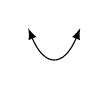
\begin{tikzpicture}
\draw[black, <->, >=latex] (-0.33, 0.5) .. controls (-0.125, 0) and (0.125, 0) .. (0.33, 0.5);
\end{tikzpicture}}

\newcommand{\CVupInc}{%
\begin{tikzpicture}
\draw[black, ->, >=latex] (0,0) .. controls (0.2, 0) and (0.4, 0.2) .. (0.5, 0.5);
\end{tikzpicture}}

\newcommand{\CVupDec}{%
\begin{tikzpicture}[rotate=270]
\draw[black, ->, >=latex] (0,0) .. controls (0.2, 0) and (0.4, 0.2) .. (0.5, 0.5);
\end{tikzpicture}}

\newcommand{\CVdown}{%
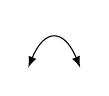
\begin{tikzpicture}
\draw[black, <->, >=latex] (-0.33, -0.5) .. controls (-0.125, 0) and (0.125, 0) .. (0.33, -0.5);
\end{tikzpicture}}

\newcommand{\CVdownInc}{%
\begin{tikzpicture}
\draw[black, ->, >=latex] (-0.5, -0.5) .. controls (-0.5, -0.3) and (-0.5, -0.1) .. (0,0);
\end{tikzpicture}}

\newcommand{\CVdownDec}{%
\begin{tikzpicture}[rotate=-90]
\draw[black, ->, >=latex] (-0.5, -0.5) .. controls (-0.5, -0.3) and (-0.5, -0.1) .. (0,0);
\end{tikzpicture}}

\begin{document}
	\noindent \hrulefill \\
	MATH-241 \hfill Pierre-Olivier Paris{\'e}\\
	Solutions Section 3-7 \hfill \semester \\\vspace*{-1cm}
	
	\noindent\hrulefill
	
	\spc
	
	\exo{2}
	\\
	Let $x$ and $y$ be those two numbers. We therefore have
		\begin{align*}
		x - y = 100 .
		\end{align*}		
	We want to minimize the product of $x$ and $y$. From the equation above, we have
		\begin{align*}
		y = x - 100 .
		\end{align*}
	The function to optimize is
		\begin{align*}
		P(x ) = xy = x (x - 100) = x^2 - 100x .
		\end{align*}	
	The derivative is 
		\begin{align*}
		P'(x) = 2x - 100
		\end{align*}
	and so $P'(x) = 0$ if $x = 50$. The second derivative is
		\begin{align*}
		P''(x) = 2 .
		\end{align*}		
	Since $P''(x) > 0$ for any $x$, we conclude that $x = 50$ is an absolute minimum. 
	
	The numbers whose product is minimum are therefore $x = 50$ and $y = -50$.		
	
	\spc
	
	\exo{8}
	\\
	Let $x$ be the width and $y$ be the heigth of the rectangle. The total area is fixed and is $1000\text{ m}^2$. This means that
		\begin{align*}
		xy = 1000 \quad \Ra \quad y = 1000/x .
		\end{align*}
	The function for the perimeter is $P = 2x + 2y$. This formulea becomes 
		\begin{align*}
		P(x) = 2x + 2000/x .
		\end{align*}
	The domain of $P$ is $x > 0$ since a negative or zero width is not possible.
	
	We take the derivative, and see that $P'(x) = 2 - 2000/x^2$. The function $P'$ is defined everywhere on $(0, \infty )$, so the critical numbers correspond to its zeros. We see that
		\begin{align*}
		P'(x) = 0 \iff x^2 = 1000 \iff x = \pm \sqrt{1000} .
		\end{align*}
	Since $x$ must be positive, we reject $-\sqrt{1000}$ and keep $\sqrt{1000}$. If we take the second derivative, we see that 
		\begin{align*}
		P''(x) = \frac{4000}{x^3}
		\end{align*}
	and, since $x > 0$, we have $P''(x) > 0$ for every $x > 0$. Thus, the number $x = \sqrt{1000}$ correspond to an absolute minimum by the second derivative test. 
	
	Finally, we have $x = \sqrt{1000}$, $y= 1000/x = \sqrt{1000}$, and the perimeter is $P = 4 \sqrt{1000} \text{ m}$.
	
	\spc
	
	\exo{14}	
	\\
	Let
		\begin{itemize}
		\item $V$: volume of the box.
		\item $b$: width of the base.
		\item $h$: height of the box.
		\item $A$: total area of the box.
		\end{itemize}	
	
	The equation of the volume of the box is
		\begin{align*}
		V = b^2 h
		\end{align*}	
	and since the volume is $32, 000\mathrm{cm}^3$, we therefore have
		\begin{align*}
		h = \frac{32000}{b^2} .
		\end{align*}	
		
	The function $A$ is the total area of the box. The box has a square base of side length $b$ with no top and four rectangular sides of sides length $b$ and $h$. Therefore, the total area is	
		\begin{align*}
		A = b^2 + 4 bh
		\end{align*}
	and using the expression of $h$, we obtain
		\begin{align*}
		A (b) = b^2 + \frac{128 000}{b} = b^2 + (128 000) b^{-1} .
		\end{align*}	
	
	We want to mimimize $A$. We have
		\begin{align*}
		A'(b) = 2b - \frac{128000}{b^2} = \frac{2b^3 - 128000}{b^2} .
		\end{align*}	
	We therefore have
		\begin{align*}
		A'(b) = 0 \iff 2b^3 - 128000 = 0 \iff b^3 = 64000 .
		\end{align*}
	Taking the third-root, we obtain
		\begin{align*}
		b = 40 .
		\end{align*}
	Taking the second derivative, we have
		\begin{align*}
		A''(b) = 2 + \frac{256000}{b^3} ..
		\end{align*}	
	We see that $A'' (b) > 0$ for any $b$. Therefore, the number $b= 40$ minimize the function $A$ (so minimize the amount of material used). 
	
	Using the link between $b$ and $h$, we find that
		\begin{align*}
		b =40\, \mathrm{cm} \quad \text{ and } \quad h = 20\,  \mathrm{cm} .
\end{align*}	

	\spc		
	
	\exo{36}
	\\
	Let $x$ (width) and $y$ (height) be the dimensions of the poster. The total area is $xy = 180$. The total of printed area is
		\begin{align*}
		A = (x - 2) (y - 3).
		\end{align*}
	Since $xy = 180$, we have $y = 180/x$ and so
		\begin{align*}
		A = (x - 2) (180/x - 3) = 3 (x - 2) (60/x - 1).
		\end{align*}
	
	The derivative of $A$ is
		\begin{align*}
		A' = 3 (60/x - 1 - 60(x - 2)/x^2)) = 3 (120/x^2 - 1) = 3 (120 - x^2)/x^2 .
		\end{align*}
	So $A' = 0$ if and only if $x = \pm \sqrt{120}$. We discard $-\sqrt{120}$ and keep $x = \sqrt{120}$. We see that $A' > 0$ when $0 < x < \sqrt{120}$ and $A' < 0$ when $x > \sqrt{120}$. So $x$ corresponds to a global maximum of $A$ on $(0, \infty )$. 
	
	So the dimensions are $x = \sqrt{120} \approx 10.95 \text{ in}$ and $y= 180/\sqrt{120} \approx 16.43 \text{ in}$. 
	
	\spc
	
	\exo{74}
	\\
	Let $l$ be the length of the pipe. Let $a$ be the angle illustrated in the figure. Let $x$ and $y$ be the sides of the right triangle with hypothenuse $l$. 
	
		\begin{center}
		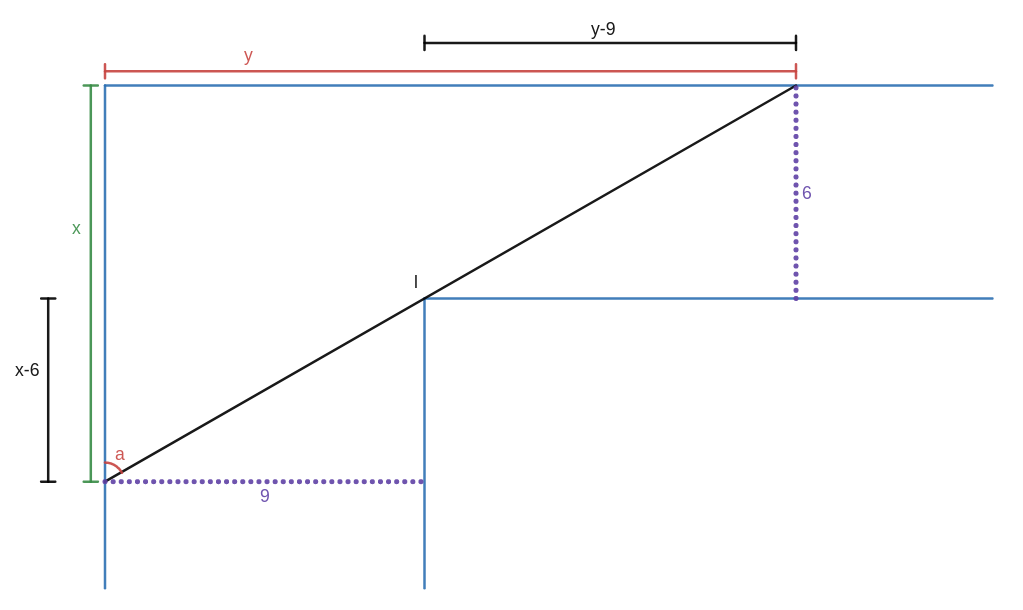
\includegraphics[scale=0.3]{number74.png}
		\end{center}
		
	From the figure, we see that $l^2 = x^2 + y^2$. We see that the angles of the two little triangles and the big triangle with side $x$ and $y$ are the same and by the similitude case AAA, the two triangles and the big one are similar. This means that
		\begin{align*}
		\frac{y}{9} = \frac{x}{x-6} \iff y = \frac{9x}{x - 6} .
		\end{align*}
	Replace this $y$ in the formulae for $l^2$ to obtain
		\begin{align*}
		l^2 = x^2 + 81 \op \frac{6}{x - 6} + 1 \fp^2 .
		\end{align*}
	
	We now take the derivative with respect to $x$. We obtain
		\begin{align*}
		2l l' = 2x - 1152 \op \frac{6}{x - 6} + 1 \fp \op \frac{1}{x - 6} \fp^2
		\end{align*}
		
		The angle $a$ is between $0$ and $\pi/2$.
	$l= x + y$
	$9/x = \sin a \Ra x = \frac{9}{\sin a} = 9 \csc a$
	$6/y = \cos a \Ra y = \frac{6}{\cos a} = 6 \sec a$
	$l = 9 \csc a + 6 \sec a$
	$l' = -9\csc a \cot a + 6 \sec a \tan a$
	$6 \sec a \tan a = 9 \csc a \cot a$
	$6 \tan^3 a = 9$
	$\tan^3 a = \frac{3}{2}$
	$a \approx 0.8527$.
	$l' < 0$
	$l \approx 21.07$
	
	\spc
	
	\exo{76}
	\\
	Let $a$ be the angle as illustrated in the picture below. To determine the maximum amount of water, we will determine the maximum area of the rain gutter. As the figure below shows, we can split the rain gutter in three simple shapes: two identical triangles and one rectangle.
		\begin{center}
		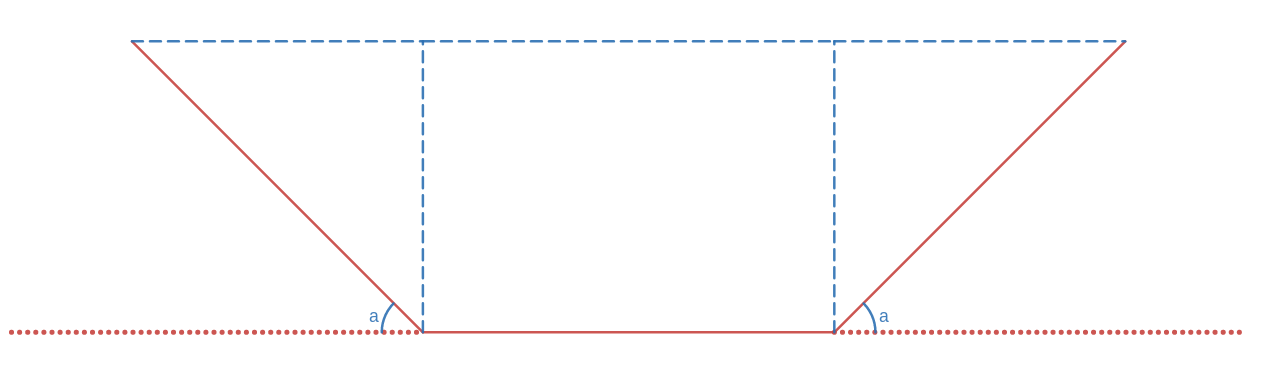
\includegraphics[scale=0.4]{number76.png}
		\end{center}
		
	The area of the triangles is 
		\begin{align*}
		A_{\Delta} = \frac{100 \cos a \sin a}{2} = 50 \cos a \sin a
		\end{align*}
	The area of the rectangle is
		\begin{align*}
		A_{\square} = 10 \cdot 10 \sin a = 100 \sin a .
		\end{align*}
	So the total area is
		\begin{align*}
		A = 2 A_{\Delta} + A_{\square} = 100 \sin a (\cos a + 1) .
		\end{align*}
	The domain of the function $a$ is between $0$ and $\pi/2$. 
	
	We take the derivative with respect to $a$. We obtain
		\begin{align*}
		A' = 100 \cos a (\cos a + 1) - 100 \sin^2 a = 100 (\cos^2 a - \sin^2 a) + 100 \cos a .
		\end{align*}
	We can replace $\cos^2 a - \sin^2 a$ by $\cos (2a)$ and we find
		\begin{align*}
		A' = 100 \cos (2a) + 100 \cos a .
		\end{align*}
	We see that 
		\begin{align*}
		A' = 0 \iff \cos 2a = -\cos a \iff \cos 2a = \cos (-a - \pi ) \iff 2a = -a + (2k-1) \pi.
		\end{align*}
	Taking $k = 0$, we see that $A' = 0$ $\iff$ $a = -\pi/3$. Taking $k= 1$, we see that $A'= 0$ $\iff$ $a = \pi/3$. This last angle is in the domain of our function $A$. 
	
	Now, $A' > 0$ when $0 < a < \pi/3$ and $A'< 0$ when $\pi/3 < a < \pi/2$. So, by the first derivative test, we see that $a = \pi/3$ corresponds to an absolute maximum on the interval $(0, \pi/2)$. The area corresponding to this angle is
		\begin{align*}
		A = 100 \sin (\pi/3) (\cos (\pi/3) + 1) \approx 129.90 \text{ m}^2 \text{ of water.}
		\end{align*}
	
	
\end{document}